%! Author = Len Washington III
%! Date = 11/6/24

% Preamble
\documentclass[
	chapter=8,
	title={Periodic Properties of the Elements},
	showanswers=true,
]{chem122notes}

%<*Chapter-8>
\chaptersetup{8}{Periodic Properties of the Elements}

% Document
\begin{document}

\maketitle

\section{Outline}\label{sec:outline-8}
\begin{itemize}
	\item History of the periodic table
	\item Effective nuclear charge
	\item Sizes of atoms and ions
	\item Trends in ionization energies
	\item Trends in electron affinities
\end{itemize}

\begin{figure}[H]
	\centering
	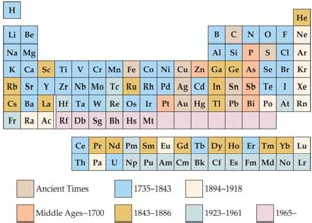
\includegraphics[width=\textwidth]{chapter8/periodic-table-dates}
	\caption{Discovery Dates of the Elements}
	\label{fig:periodic-table-dates}
\end{figure}

\section{Development of the Periodic Table}\label{sec:development-of-the-periodic-table}
\begin{itemize}
	\item Mendeleev's insistence that elements with similar properties be listed in the same group lead him to leave several blanks in the periodic table.
	\item For example, Mendeleev predicted some properties of now what is called Germanium based on the fact that it is in the same group as Silicon.
	Silicon was discovered almost 100 years before that of Germanium!
	\item Once germanium was discovered, its observed properties matched exceptionally well with Mendeleev's predictions (see the table on the next slide).
\end{itemize}

\begin{table}[H]
	\centering
	\caption{Comparison of the Properties of Eka-Silicon (\emph{``under'' silicon}) Predicted by Mendeleev with the Observed Properties of Germanium}
	\label{tab:silicon-properties}
	\begin{tabular}{*{3}{p{0.3\textwidth}}}
		\textbf{Property} & \textbf{Mendeleev's Predictions for Eka-Silicon (made in 1871)} & \textbf{Observed Properties of Germanium (discovered in 1886)}\\
		\hline
		Atomic weight & 72 & 72.59\\
		Density (g/$\mbox{cm}^{3}$) & 5.5 & 5.35\\
		Specific heat (J/g$\times$K) & 0.305 & 0.309\\
		Melting point (\textdegree{}C) & High & 947\\
		Color & Dark gray & Grayish white\\
		Formula of oxide & \ce{XO2} & \ce{GeO2}\\
		Density of oxide (g/$\mbox{cm}^{3}$) & 4.7 & 4.70\\
		Formula of chloride & \ce{XCl4} & \ce{GeCl4}\\
		Boiling point of chloride (\textdegree{}C) & A little under 100 & 84\\
		\hline
	\end{tabular}
\end{table}

\definition{Periodic law 1860--1870's (Mendeleev and Meyer)}{\emph{A periodic repetition of physical and chemical properties} occurs when the elements are arranged in order of increasing atomic \textit{weight [\emph{number}]}}

\begin{figure}[H]
	\centering
	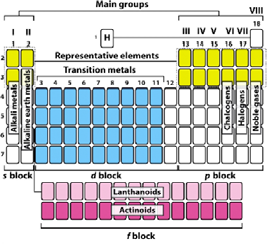
\includegraphics[width=\textwidth]{chapter8/periodic-table-2}
	\caption{}
	\label{fig:periodic-table-2}
\end{figure}

\section{Ordering by Atomic Weight}\label{sec:ordering-by-atomic-weight}
\textbf{Inconsistencies in ordering by atomic weight:}
\begin{itemize}\newcommand{\weights}[3]{\ce{#1} (#2 amu; $Z=#3$)}
	\item \weights{Co}{58.93}{27} and \weights{Ni}{58.69}{28}
	\item \weights{Ar}{39.95}{18} and \weights{K}{39.10}{19}
	\item \weights{Te}{127.60}{52} and \weights{I}{126.90}{53}
\end{itemize}
\emph{However, all of the above are correctly ordered by atomic number, $Z$ (i.e., the number of protons).}

\section{Development of Periodic Table}\label{sec:development-of-periodic-table}
\begin{itemize}
	\item Elements in the same group generally have similar chemical properties.
	\item However, physical properties are not necessarily similar.
	\item For example, even though Oxygen and Sulfur are in the same group (6A), Oxygen is a colorless gas, while Sulfur is a yellow solid under normal conditions.
\end{itemize}

\section{But why do elements in the same group have similar properties?}\label{sec:but-why-do-elements-in-the-same-group-have-similar-properties?}
\begin{itemize}
	\item Underlying valence electronic structure is the same (almost) for elements of a group:
	\begin{itemize}
		\item e.g., alkaline earth metals (Group 2) metals are all
		\begin{electronstructure}
			[Noble Gas] $\mbox{ns}^{2}$
		\end{electronstructure}
		\item halogens (Group 17) are all
		\begin{electronstructure}
			[Noble Gas] $\mbox{ns}^{2}\mbox{np}^{5}$
		\end{electronstructure}
	\end{itemize}
	\item So, broadly speaking, elements in the same group \textit{should} have similar chemistry
	\item But why do properties like \emph{atomic size}, \emph{ionization energies} and \emph{electron affinity} vary from group to group?.
\end{itemize}

\section{Effective Nuclear Charge}\label{sec:effective-nuclear-charge}
\begin{minipage}[m]{0.5\textwidth}
	\begin{figure}[H]
		\centering
		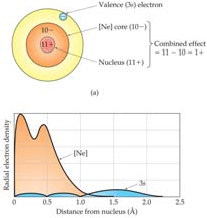
\includegraphics[width=\textwidth]{chapter8/effective-nuclear-charge}
		\caption{Effective Nuclear Charge}
		\label{fig:effective-nuclear-charge}
	\end{figure}
\end{minipage}\hfill%
\begin{minipage}[m]{0.45\textwidth}
	\begin{itemize}
		\item In a many-electron atom, electrons are both attracted to the nucleus and repelled by other electrons.
		\item The nuclear charge that an electron experiences depends on both factors.
		\item The effective nuclear charge, $Z_{eff}$, is found this way:
		\begin{equation}
			Z_{eff} = Z - \sigma
			\label{eq:effective-nuclear-charge}
		\end{equation}
		where $Z$ is the atomic number and $\sigma$ is the screening constant, usually close to the number of inner/core electrons.
		\item $Z_{eff}$ is always less than $Z$ (atomic number) due to shielding!
		\item Electrons in the same shell don't screen one another very well.
	\end{itemize}
\end{minipage}

\section{What is the Size of an Atom?}\label{sec:what-is-the-size-of-an-atom?}
\begin{minipage}[m]{0.4\textwidth}
	\begin{figure}[H]
		\centering
		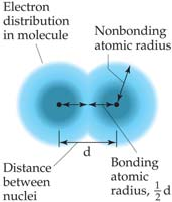
\includegraphics[width=\textwidth]{chapter8/atom-size}
		\caption{Atom Size}
		\label{fig:atom-size}
	\end{figure}
\end{minipage}\hfill%
\begin{minipage}[m]{0.6\textwidth}
	\begin{itemize}
		\item The bonding atomic radius is defined as $\frac{1}{2}$ of the distance between covalently bonded nuclei.
	\end{itemize}
\end{minipage}

\begin{minipage}[m]{0.4\textwidth}
	\begin{figure}[H]
		\centering
		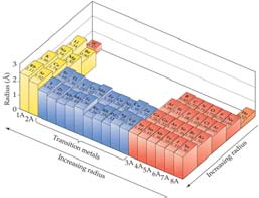
\includegraphics[width=\textwidth]{chapter8/periodic-table-sizes}
		\caption{Sizes of Atoms}
		\label{fig:periodic-table-sizes}
	\end{figure}
\end{minipage}\hfill%
\begin{minipage}[m]{0.6\textwidth}
	\begin{itemize}
		\item Bonding atomic radii tend to:
		\begin{enumerate}[label=(\Alph*)]
			\item decrease from left to right across a row (\emph{due to increasing $Z_{eff}$}).
			\item increase from top to bottom of a column (\emph{due to increasing value of $n$}).
		\end{enumerate}
	\end{itemize}
\end{minipage}

\section{Estimating Bond Lengths}\label{sec:estimating-bond-lengths}
\begin{itemize}
	\item Atomic radii allows one to estimate bond lengths.
	\item Example, estimate the carbon-chlorine bond length in carbon tetrachloride, \ce{CCl4}.
	\textcolor{red}{
		Atomic radius of \ce{C}: 0.77 \si{\angstrom}\\
		Atomic radius of \ce{Cl}: 0.99 \si{\angstrom}\\
		Intenuclear bond length = 0.77 \si{\angstrom} + 0.99 \si{\angstrom} = 1.76 \si{\angstrom}\\
	}
	\item The experimentally determined carbon-chlorine bond length in carbon tetrachlroide is actually 1.77 \si{\angstrom}.
\end{itemize}

\section{Radii of Cations and Anions}\label{sec:radii-of-cations-and-anions}
\begin{minipage}[m]{0.6\textwidth}
	\begin{figure}[H]
		\centering
		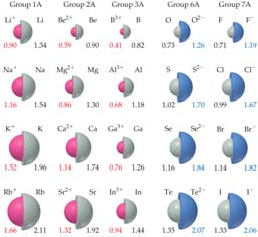
\includegraphics[width=\textwidth]{chapter8/cation-anion-radii}
		\caption{Radii of Cations and Anions}
		\label{fig:cation-anion-radii}
	\end{figure}
\end{minipage}\hfill%
\begin{minipage}[m]{0.4\textwidth}
	\begin{itemize}
		\item Cations are smaller than parent neutral atoms (e.g., \ce{Li+} is smaller than \ce{Li}.) \emph{Why?}
		\item Increased $Z_{eff}$ upon electron removal.
		\item Anions are larger than parent neutral atoms (e.g., \ce{I-} is larger than \ce{I}.) \emph{Why?}
		\item Increased electron-electron repulsions upon electron addition, causing electrons to spread out more in space.
		\item \definition{Ions with the same charge}{ion size increases going down a group \emph{due to increasing values of $n$}}.
		\item For example, a \ce{Sr^2+} ion (radius = 1.32 \si{\angstrom}) is larger than a \ce{Ca^2+} ion (radius = 1.14 \si{\angstrom}).
	\end{itemize}
\end{minipage}

\section{Sizes of Isoelectronic Ions}\label{sec:sizes-of-isoelectronic-ions}
\begin{itemize}
	\item In an \emph{isoelectronic series}, ions have the same number of electrons.
	\item Ionic size decreases with an increasing nuclear charge ($Z_{eff}$).
\end{itemize}
\begin{figure}[H]
	\centering
	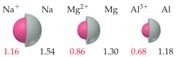
\includegraphics[width=0.45\textwidth]{chapter8/isoelectronic-ions-1}
	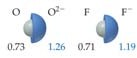
\includegraphics[width=0.45\textwidth]{chapter8/isoelectronic-ions-2}
	\caption{Sizes of Isoelectronic Ions}
	\label{fig:sizes-of-isoelectronic-ions}
\end{figure}

\section{Ionization Energy}\label{sec:ionization-energy}
\begin{itemize}
	\item \definition{Ionization energy}{energy required to remove an electron from a gaseuos species.}
	\item The first ionization energy is the energy required to remove the first electron.
	\item The second ionization energy is the energy required to remove the second electron, etc.
	\begin{equation*}
	\begin{aligned}
		\ce{Mg} \stackrel{IE_{1} = 738 \frac{kJ}{mol}}{\longrightarrow} \ce{Mg+} \stackrel{IE_{2} = 1451 \frac{kJ}{mol}}{\longrightarrow} \ce{Mg^2+}\\
	\end{aligned}
	\end{equation*}
	\item It requires more energy to remove each successive electron.
	\item When all valence electrons have been removed, the ionization energy takes a large leap.
	\item Ionization energies for all elements can be found at: \url{https://www.webelements.com}
\end{itemize}

\begin{figure}[H]
	\centering
	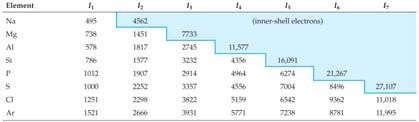
\includegraphics[width=\textwidth]{chapter8/ionization_energy}
	\caption{Ionization Energy}
	\label{fig:ionization-energy}% TODO: Replace this with LaTeX table
\end{figure}

\section{Trends in First Ionization Energies}\label{sec:trends-in-first-ionization-energies}
\begin{minipage}[m]{0.5\textwidth}
	\begin{figure}[H]
		\centering
		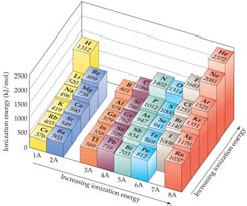
\includegraphics[width=\textwidth]{chapter8/periodic-table-ionizations}
		\caption{Periodic Table Ionization Energies}
		\label{fig:periodic-table-ionizations}
	\end{figure}
\end{minipage}\hfill
\begin{minipage}[m]{0.5\textwidth}
	\begin{itemize}
		\item As one goes down a group, less energy is required to remove the first electron.
		\begin{itemize}
			\item For atoms in the same group, $Z_{eff}$ is essentially the same, but the valence electrons are farther from than nucleus (i.e., increasing value of $n$).
		\end{itemize}
	\end{itemize}
\end{minipage}

\begin{minipage}[m]{0.5\textwidth}
	\begin{figure}[H]
		\centering
		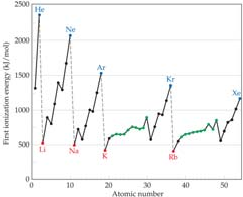
\includegraphics[width=\textwidth]{chapter8/ionization-energy-trends}
		\caption{Trends in Ionization Energy}
		\label{fig:trends-in-ionization-energy}
	\end{figure}
\end{minipage}\hfill
\begin{minipage}[m]{0.5\textwidth}
	\begin{itemize}
		\item Generally, as one goes across a row/period, it becomes more difficult to remove an electron.
		\begin{itemize}
			\item As you go from left to right $\Rightarrow Z_{eff}$ increases!
		\end{itemize}
	\end{itemize}
\end{minipage}

\begin{minipage}[t]{0.5\textwidth}
	\begin{figure}[H]
		\centering
		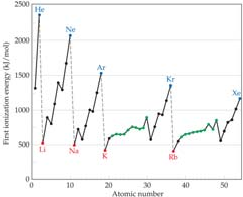
\includegraphics[width=\textwidth]{chapter8/ionization-energy-trends-discontinuities}% TODO: Draw the circles on the discontinuities
		\caption{Discontinuities in Trends in Ionization Energy}
		\label{fig:trends-in-ionization-energy-discontinuities}
	\end{figure}
\end{minipage}\hfill
\begin{minipage}[t]{0.5\textwidth}
	\begin{itemize}
		\item However, there are two apparent discontinuities in this trend.
		\item The first occurs between Groups IIA (2) and IIIA (13).
		\item In this case, the electron is removed from a $p$-orbital rather than an $s$-orbital.
		\begin{itemize}
			\item The electron removed is further from the nucleus.
			\item There is also a small amount of repulsion by the $s$ electrons.
		\end{itemize}
		\item The second occurs between Groups VA (15) and VIA (16).
		\begin{itemize}
			\item The electron removed comes from a doubly occupied orbital.
			\item Repulsion from the other electron in the orbital aids in the removal.
		\end{itemize}
	\end{itemize}
\end{minipage}

%Account for the decrease in ionization energy in going from nitrogen (N) to oxygen (O) despite the increase in effective nuclear charge ($Z_{eff}$).
%\begin{answer}
%\end{answer}

\section{Electron Affinity}\label{sec:electron-affinity}
Electron affinity is the energy change accompanying the addition of an electron to a gaseous atom:
\begin{equation*}
\begin{aligned}
	\ce{CL(g) + e- ->  Cl-(g)}\ \ \ \ \ E_{a} = -349 \frac{\mbox{kJ}}{\mbox{mol}}
\end{aligned}
\end{equation*}
Energy is typically released when an electron is added to a gaseous atom.
The process is said to be \emph{exothermic}, so the energy has a negative sign associated with it.\\

The electron affinity of lithium is a negative value, whereas the electron affinity of Beryllium is a positive value.
Use electron configuration to account for this observation.

\section{Trends in Electron Affinity}\label{sec:trends-in-electron-affinity}
\begin{minipage}[m]{0.5\textwidth}
	\begin{figure}[H]
		\centering
		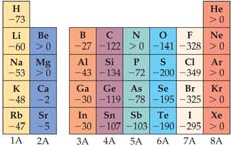
\includegraphics[width=\textwidth]{chapter8/electron-affinity}
		\caption{Trends in Electron Affinity}
		\label{fig:trends-in-electron-affinity}
	\end{figure}
\end{minipage}\hfill
\begin{minipage}[m]{0.5\textwidth}
	\begin{itemize}
		\item In general, electron affinities become more exothermic/more negative as you go from left to right across a period.
	\end{itemize}
\end{minipage}
\begin{minipage}[m]{0.5\textwidth}
	\begin{figure}[H]
		\centering
		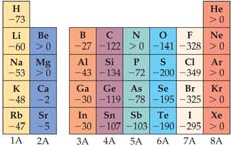
\includegraphics[width=\textwidth]{chapter8/electron-affinity} % TODO: Add the discontinuities for this too
		\caption{Discontinuities in Trends in Electron Affinity}
		\label{fig:trends-in-electron-affinity-discontinuities}
	\end{figure}
\end{minipage}\hfill
\begin{minipage}[m]{0.5\textwidth}
	\begin{itemize}
		\item However, there are two discontinuities in this trend.
	\end{itemize}
\end{minipage}

\begin{itemize}
	\item This first occurs between Groups IA and IIA.
	\begin{itemize}
		\item The added electron must go in a $p$-orbital, not an $s$-orbital.
		\item The electron is farther from nucleus and feels repulsion from the $s$-electrons.
	\end{itemize}
	\item The second occurs between Groups IVA and VA.
	\begin{itemize}
		\item Group VA has no empty orbitals.
		\item The extra electron must go into an already occupied orbital, creating repulsion.
	\end{itemize}
\end{itemize}

%</Chapter-8>
\end{document}
